\documentclass{beamer}
\usepackage{ragged2e}
\usepackage[frenchb]{babel}
\usetheme[subsectionpage=progressbar]{metropolis}
\usepackage{fancyvrb}
\usepackage{graphicx}
\usepackage{listings}
\usepackage{xcolor}

\setcounter{tocdepth}{1}
\apptocmd{\frame}{}{\justifying}{} % Allow optional arguments after frame.

\colorlet{punct}{red!60!black}
\definecolor{background}{HTML}{EEEEEE}
\definecolor{delim}{RGB}{20,105,176}
\colorlet{numb}{magenta!60!black}

\lstdefinelanguage{json}{
  basicstyle=\normalfont\ttfamily,
  numbers=left,
  numberstyle=\scriptsize,
  stepnumber=1,
  numbersep=8pt,
  showstringspaces=false,
  breaklines=true,
  frame=lines,
  backgroundcolor=\color{background},
  literate=
  *{0}{{{\color{numb}0}}}{1}
  {1}{{{\color{numb}1}}}{1}
  {2}{{{\color{numb}2}}}{1}
  {3}{{{\color{numb}3}}}{1}
  {4}{{{\color{numb}4}}}{1}
  {5}{{{\color{numb}5}}}{1}
  {6}{{{\color{numb}6}}}{1}
  {7}{{{\color{numb}7}}}{1}
  {8}{{{\color{numb}8}}}{1}
  {9}{{{\color{numb}9}}}{1}
  {:}{{{\color{punct}{:}}}}{1}
  {,}{{{\color{punct}{,}}}}{1}
  {\{}{{{\color{delim}{\{}}}}{1}
  {\}}{{{\color{delim}{\}}}}}{1}
  {[}{{{\color{delim}{[}}}}{1}
  {]}{{{\color{delim}{]}}}}{1},
}

\title{Quelques notions et outils indispensables au dev Web}
\date{}
\author{Lionel \textsc{Kitihoun}}

\begin{document}
\begin{frame}[plain]
\maketitle
\end{frame}

\begin{frame}{Sommaire}
\tableofcontents
\end{frame}

\section{Web et HTTP}
\subsection{Généralités}

\begin{frame}{Web}
Système hypertexte public fonctionnant sur Internet. Il permet de consulter, avec un navigateur, des pages ou médias accessibles sur des sites\footnote{\url{https://fr.wikipedia.org/wiki/World\_Wide\_Web}}.
\end{frame}

\begin{frame}{Autres services fonctionnant grâce à Internet}
\begin{itemize}
  \item Transfert de fichiers (FTP)
  \item Méssagerie électronique (SMTP)
  \item VoIP
  \item etc.
\end{itemize}
\end{frame}

\begin{frame}{HTTP}
\begin{itemize}
  \item Définition ?
\uncover<2-4>{
  \item Hypertext Transfer Protocol.
}
\uncover<3-4>{
  \item Protocole de communication client-serveur développé pour le World Wide Web \footnote{\url{https://fr.wikipedia.org/wiki/Hypertext_Transfer_Protocol}}.
}
\uncover<4>{
  \item HTTPS est la variante sécurisée par l'usage des protocoles Transport Layer Security (TLS).
}
\end{itemize}
\end{frame}

\begin{frame}{HTTP}
\setbeamercovered{transparent}
\begin{itemize}
  \item Tout développeur se doit de le connaître.
  \pause
  \item Parce qu'il est fort probable qu'un jour vous devrez vous y frotter.
  \pause
  \item Web, mobile, système, IoT...
\end{itemize}
\end{frame}

\subsection{Méthodes}
\begin{frame}{Méthodes}
Le protocole fonctionne sur la base de \textbf{verbes} ou \textbf{méthodes}, qui indiquent le type de requête initiée par le client.

\pause
Il y en a plusieurs, notamment:
\begin{itemize}
  \item GET
  \item HEAD
  \item POST
  \item PUT
  \item PATCH
  \item DELETE
  \item OPTIONS
\end{itemize}
\end{frame}

\begin{frame}{Petite explication technique}
Un serveur met à disposition de ses clients des ressources, accessibles via une URL. Au début du web, les ressources étaient généralement des pages HTML, des documents, des images ou des vidéos.

Avec l'évolution de web, les ressources peuvent représenter beaucoup d'autres choses, les entités stockées dans une base de données, des relevés d'impôts, des données de natures diverses.
\end{frame}

\begin{frame}{GET}
C'est la méthode la plus courante pour demander la représentation d'une ressource. Elle ne doit entraîner aucune modification côté serveur.
\end{frame}

\begin{frame}{HEAD}
Cette méthode ne demande que des informations (métadonnées) sur la ressource, sans demander la ressource elle-même.

Utile par exemple pour la mise en cache, pour savoir si une ressource a été modifiée par exemple.
\end{frame}

\begin{frame}{POST}
Cette méthode est utilisée pour transmettre des données en vue d'un traitement.
\end{frame}

\begin{frame}{PUT}
Cette méthode est utilisée pour remplacer intégralement une ressource.
\end{frame}

\begin{frame}{PATCH}
Cette méthode est utilisée pour modifier partiellement une ressource.
\end{frame}

\begin{frame}{DELETE}
Comme son nom ne l'indique pas, cette méthode est utiliser pour supprimer une ressource sur le serveur.

Bien entendu, le serveur devra s'assurer que le client qui requiert cette action en a le droit.
\end{frame}

\begin{frame}{OPTIONS}
Cette méthode permet d'obtenir les options de communication d'une ressource ou du serveur en général.
\end{frame}

\subsection{Codes de réponse HTTP}
\begin{frame}{Codes de réponse HTTP}
  Les codes de statut de réponse HTTP sont utilisés par le serveur pour indiquer si une requête HTTP a été exécutée avec succès ou non.

  Les codes de réponse sont regroupées en cinq classes. Elles apparaissent dans l'entête de la réponse.
\end{frame}

\begin{frame}{Classes de réponse HTTP}
\setbeamercovered{transparent}
\begin{itemize}
\uncover<1,6>{
  \item Les réponses informatives (100 - 199).
}
\uncover<2,6>{
  \item Les réponses de succès (200 - 299).
}
\uncover<3,6>{
  \item Les messages de redirection (300 - 399).
}
\uncover<4,6>{
  \item Les erreurs du client (400 - 499).
}
\uncover<5->{
  \item Les erreurs du serveur (500 - 599)
}
\end{itemize}
\end{frame}

\subsection{Entêtes HTTP}

\begin{frame}{Entêtes HTTP}
Elles permettent au client et aux serveurs d'ajouter des informations supplémentaires aux messages HTTP.

Certaines entêtes sont propres aux requêtes, d'autres aux réponses. D'autres peuvent être présentes dans les deux.
\end{frame}

\begin{frame}{Entêtes fréquentes}
\begin{itemize}
\only<1>{
  \item \textbf{Content-Type}\\
     Utilisé pour indiquer le type MIME du corps du message.
}
\only<2>{
  \item \textbf{Content-Length} \\
    Utilisé pour indiquer la longueur (en octets) du corps du message.
}
\only<3>{
  \item \textbf{Accept} \\
    Utilisé par le client pour indiquer les types MIME qu'il souhaite pour la réponse.
}
\only<4>{
  \item \textbf{Location} \\
    Utilisé par le serveur pour indiquer une redirection.
}
\only<5>{
  \item \textbf{Host} \\
    Utilisé par le client pour indiquer à quelle site la requête est envoyée.\\
    Plusieurs sites ou applications peuvent être hébergées sur un même serveur.\\
    Cet entête est donc très important.
}
\only<6>{
  \item \textbf{Authorization} \\
  Utilisé pour l'authentification. Utilisé par exemple par les web services et les APIs web pour la gestion des accès.
}

\only<7>{
  \item \textbf{Cookie}, \textbf{Set-Cookie} \\
    Pour la gestion des cookies (Miam).
}
\end{itemize}
\end{frame}

\subsection{Cookies}
\begin{frame}{Cookies I}
  Un cookie est une information générée par un serveur web et stocké chez le client suite à une requête.
  
  Ils sont utilisés à des fins de personnalisation du contenu, d'identification des utilisateurs, pour la publicité et le suivi des individus sur le web.
\end{frame}

\begin{frame}{Cookies II}
  HTTP est un protocole sans état. Le serveur n'a aucun moyen de savoir que certaines requêtes proviennent d'un même client.
  
  Les cookies étaient utilisés par les sites pour faire le lien entre les requêtes successives d'un utilisateur. Le serveur ajoute des cookies à une réponse et le client renvoie les mêmes cookies lors d'une autre requête. Le serveur peut ainsi les reconnaître.
\end{frame}

\begin{frame}{Cookies III}
Malheureusement, l'utilisation des cookies a été pervertie.

Jetez un\oe{}il aux cookies stockés dans votre navigateur. ;)
\end{frame}

\subsection{Faire des requêtes HTTP}
\begin{frame}{S'amuser à faire des requêtes HTTP}
\setbeamercovered{transparent}
Il existe de nombreux outils pouvant aider à lancer des requêtes HTTP vers un serveur.
\begin{itemize}
\uncover<1,4>{
  \item \textbf{Votre navigateur web}\\
  Vous déclenchez un nombre incalculable de requêtes quand vous naviguez.
}
\uncover<2,4>{
  \item \textbf{Les outils destinés aux développeurs} \\
  \begin{itemize}
    \item Postman
    \item Insomnia
  \end{itemize}
}
\uncover<3,4>{
  \item \textbf{Les outils en ligne de commande}\\
  \begin{itemize}
    \item telnet
    \item curl (la référence)
    \item netcat (ncat)
    \item httpie
  \end{itemize}
}
\end{itemize}
\end{frame}

\begin{frame}{Quelques requêtes HTTP}
\begin{itemize}
  \item GET
  \item HEAD
  \item POST
\end{itemize}
\end{frame}

\section{REST et OpenAPI}
\begin{frame}{REST}
REST
\begin{itemize}
\only<1>{
  \item REpresentational State Transfer
}
\only<2>{
  \item Style d'architecture logicielle définissant un ensemble de contraintes à utiliser pour créer des services web\footnote{\url{https://fr.wikipedia.org/wiki/Representational\_state\_transfer}}
}
\only<3>{
  \item Les services web REST permettent aux systèmes effectuant des requêtes de manipuler des ressources web via leurs représentations textuelles à travers un ensemble d'opérations uniformes et prédéfinies sans état.
}
\end{itemize}
\end{frame}

\begin{frame}{REST et HTTP}
REST est souvent utilisé avec HTTP.

Un mapping est donc utilisé entre les méthodes HTTP et les opérations CRUD sur les entités manipulées.
\begin{itemize}
  \item GET
  \item POST
  \item PUT/PATCH
  \item DELETE
\end{itemize}
\end{frame}

\begin{frame}{Exemple de ressources REST}
\begin{itemize}
  \item GET /persons
  \item POST /persons
  \item GET /persons/1
  \item PUT /persons/1
  \item PATCH /persons/1
  \item DELETE /persons/1
\end{itemize}
\end{frame}

\begin{frame}{Open API Spec}
Standard utilisé pour décrire les opérations offertes par une API ou web services.

Le format utilisé pour la description est le YAML (ou le JSON).
\end{frame}

\begin{frame}[fragile]
\frametitle{Exemple}
\begin{Verbatim}[fontsize=\scriptsize]
openapi: 3.1.0
info:
  title: Tic Tac Toe
  description: This API allows to play Tic Tac Toe.
  version: 1.0.0
paths:
  # Whole board operations
  /board:
    get:
      summary: Get the whole board
      description: Retrieves the current state of the board and the winner.
      responses:
        "200":
          description: "OK"
          content:
...
\end{Verbatim}  
\end{frame}

\section{Outils pour tester et développer des APIs}
\begin{frame}{Postman}
\begin{center}
  
\includegraphics[scale=0.2]{images/postman-logo.png}
\end{center}
\end{frame}

\begin{frame}{Insomnia}
\begin{center}
  
\includegraphics[scale=0.1]{images/insomnia-logo.png}
\end{center}
\end{frame}

\begin{frame}{Swagger}
\begin{center}
  
\includegraphics[scale=0.18]{images/swagger.png}
\end{center}
\end{frame}

\section{Git}

\begin{frame}{Git}
\begin{center}
  
\includegraphics[scale=0.25]{images/git-logo.png}
\end{center}
\end{frame}

\begin{frame}{Git}
\setbeamercovered{transparent}
\begin{itemize}
\uncover<1->{
  \item Logiciel de gestion de versions décentralisé
}
\uncover<2->{
  \item Logiciel libre
}
\uncover<3->{
  \item Créé par Linus Torvalds
}
\uncover<3->{
  \item Site web : \url{https://git-scm.com}
}
\end{itemize}
\end{frame}

\begin{frame}{Fonctionnement}
\begin{center}
  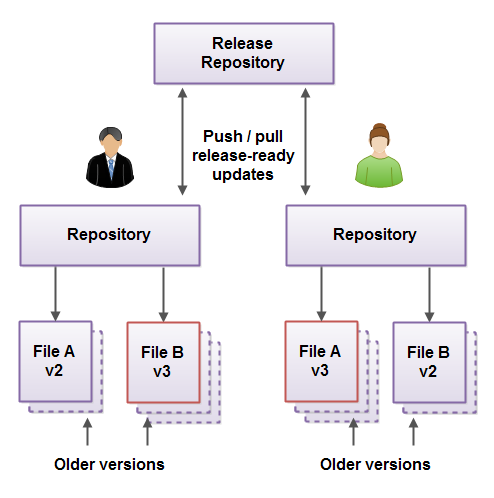
\includegraphics[scale=0.5]{images/git-release-repository.png}
\end{center}
\end{frame}

\begin{frame}{Commandes courantes de Git}
\begin{itemize}
\only<1>{
  \item \textbf{git init}\\
  Pour initialiser un nouveau dépôt.
}
\only<2>{
  \item \textbf{git add} \\
  Pour enregistrer des changements.
}
\only<3>{
  \item \textbf{git commit} \\
  Utilisé valider les changements.
}
\only<4>{
  \item \textbf{git push} \\
  Pour pousser son travail vers le dépôt central.
}
\only<5>{
  \item \textbf{git pull} \\
  Pour se synchroniser avec le dépôt central.
}
\only<6>{
  \item \textbf{git clone} \\
  Pour faire une copie d'un dépôt.
}
\end{itemize}
\end{frame}

\begin{frame}{Plateformes}
\begin{itemize}
\only<1>{
  \item \textbf{GitHub} \\
    Propriétaire, mais accessible
    \vspace{15pt}
    \begin{center}
      \includegraphics[scale=0.2]{images/github.png}
    \end{center}
}
\only<2>{
  \item \textbf{GitLab} \\
    Opensource
    \begin{center}
      \includegraphics[scale=0.3]{images/gitlab.png}
    \end{center}
}
\end{itemize}
\end{frame}

\begin{frame}{Pull request}
  On parle de \textbf{pull request} lorsqu'un développeur demande que les changements ou ajouts qu'il a effectués sur sa copie soient intégrés dans le dépôt principal.

  Le propriétaire du dépôt peut accepter (après validation des modifications) ou non la requête.

  Le rejet d'un \textbf{pull request} donne parfois naissance à un \textbf{fork}.
\end{frame}

\section{Composer}
\begin{frame}{Composer}
\begin{center}
  
\includegraphics[scale=1.5]{images/composer.png}
\end{center}
\end{frame}

\begin{frame}{Composer}
\begin{itemize}
  \item Gestionnaire de dépendances pour les projets PHP.
  \item Inspiré de NPM (Node Package Manager).
  \item Installe les paquets depuis \url{https://packagist.org/}.
\end{itemize}
\end{frame}

\begin{frame}[fragile]
\frametitle{Utilisation I}
  1. Déclarer les dépendances dans un fichier \texttt{composer.json} à la racine du projet.
  \begin{lstlisting}[language=json]
    {
      "require": {
        "psr/log": "1.3.2",
        "fakerphp/faker": "1.*",
        "guzzlehttp/guzzle": "^7.4.0"
      }
    }
  \end{lstlisting}
\end{frame}

\begin{frame}{Utilisation II}
  2. Installer Composer (globalement ou en local).
\end{frame}

\begin{frame}[fragile]{Utilisation III}
  3. Installer les paquets avec la commande :
  \begin{Verbatim}
    php composer.phar install # Installation locale
    composer install # Installation globale
  \end{Verbatim}
\end{frame}

\begin{frame}[fragile]{Utilisation IV}
  4. Charger automatiquement les dépendances à l'exécution.
  \begin{verbatim}
    require 'vendor/autoload.php';
  \end{verbatim}
\end{frame}

\section{MVC, PHP et Laravel}

\subsection{MVC}
\begin{frame}{MVC}
Patron de conception qui promeut la séparation du code des applications en trois parties :
\begin{itemize}
  \item Le modèle, qui représente les données manipulées et les traitements métier associés.
  \item La vue, l'interface de l'application avec laquelle l'utilisateur interagit.
  \item Le contrôleur, qui détermine les traitements à éffectuer en fonctions des actions de l'utilisateur.
\end{itemize}
\end{frame}

\begin{frame}{Origines et utilisation actuelle du MVC}
Le MVC a été créé pour faciliter le développement des applications graphiques. Il est par exemple utilisé par Swing et Qt.

Mais il a été appliqué avec succès dans le domaines des applications web car il facilite grandemant le processus de développement et permet le partge des tâches entre les devs.
\end{frame}

\begin{frame}{Frameworks MVC}
\begin{itemize}
  \item PHP : Laravel, Symfony.
  \item Python : Django.
  \item Ruby : Ruby on Rails.
  \item Java : Sping.
\end{itemize}
\end{frame}

\subsection{Laravel}
\begin{frame}{Laravel}
\begin{itemize}
  \item Framework MVC écrit en PHP très populaire.
  \item \url{https://laravel.com}
    \vspace{10pt}
    \begin{center}
      
\includegraphics[scale=0.3]{images/laravel.png}
    \end{center}
\end{itemize}
\end{frame}

\begin{frame}[fragile]
\frametitle{Installation}
\begin{footnotesize}
  \begin{Verbatim}
    composer create-project --prefer-dist laravel/laravel my-app
    cd my-app
    php artisan serve
  \end{Verbatim}
\end{footnotesize}
\end{frame}

\begin{frame}[fragile]
\frametitle{Installation d'une version spécifique}
\begin{footnotesize}
  \begin{Verbatim}
    composer create-project --prefer-dist laravel/laravel my-app 5.6
    cd my-app
    php artisan serve
  \end{Verbatim}
\end{footnotesize}
\end{frame}

\begin{frame}[fragile]
  \frametitle{Installeur Laravel}
  \begin{footnotesize}
    \begin{Verbatim}
      composer global require laravel/installer
      laravel new my-app
      cd my-app
      php artisan serve
    \end{Verbatim}
  \end{footnotesize}
\end{frame}

\begin{frame}{Page d'accueil par défaut}
\begin{center}
  
\includegraphics[scale=0.4]{images/laravel-welcome-page.png}
\end{center}
\end{frame}
\end{document}
